\section{Tarea}

\subsection{Objetivo}

\begin{itemize}
    \item Introducción al lenguaje Qt.
\end{itemize}



\subsection{Problema propuesto: }

\begin{enumerate}[label={[\arabic*]}]
    \item Crear una interface gráfica (que implemente señales y slots) que muestre una lista de nombres de colores, al dar clic sobre alguno que se muestre un Label o un Text con el nombre del color.
    \item Averiguar la implementación por signals y Slots, para comunicar los objetos del formulario del Task.ui (por ejemplo una caja de texto, o un Label) desde el MainWindows.h y CPP.
\end{enumerate}




\section{Equipos, materiales y temas utilizados}

\begin{itemize}
    \item Subsistema de Windows para Linux (WSL) con Ubuntu.
    \item Sistema operativo: Microsoft Windows [Versión 10.0.26100.6584]
    \item TeX Live 2025
    %\item Strawberry Perl (requerido por MiKTeX para la ejecución de scripts auxiliares en la compilación de ciertos paquetes).
    \item Helix 25.01.1 (e7ac2fcd)
    \item Visual Studio Code 1.104.0 x64
    \item Git version 2.41.0.windows.1
    \item Cuenta activa en GitHub para la gestión de repositorios remotos.
    \item Qt Creator
    \item Leguaje de programación C++
    \item Librería Qt
\end{itemize}




\section{URL de Repositorio Github}

\begin{itemize}
    \item URL del Repositorio GitHub para clonar o recuperar.
    \item \url{https://github.com/yhuayhuahi/Teo.git}
    \item URL para el laboratorio (\itemPracticeNumber) en el Repositorio GitHub.
    \item \url{https://github.com/yhuayhuahi/Teo/tree/main/laboratorios/lab\itemPracticeNumber}
\end{itemize}




\section{Desarrollo de las actividades}

\subsection {Actividad 01: Implementación en C++ con Qt}

\subsubsection {Función Main en C++}

A continución se muestra la función main implementada en C++ utilizando la librería Qt para crear una aplicación gráfica que muestra una lista de colores y actualiza un label con el nombre del color seleccionado.

\begin{lstlisting}[style=cpp-style, caption={Función Main en cpp - Primera implementación}]
#include "mainwindow.h"
#include <QApplication>

int main(int argc, char *argv[])
{
    QApplication app(argc, argv);

    MainWindow w;
    w.show();

    return app.exec();
}
\end{lstlisting}



\subsubsection {Clase MainWindow en C++}

A continuación se muestra el archivo de encabezado (header) de la clase MainWindow en C++ que define la interfaz gráfica y los elementos necesarios para la aplicación.

\begin{lstlisting}[style=cpp-style, caption={Header de la clase MainWindow en C++}]
#ifndef MAINWINDOW_H
#define MAINWINDOW_H

#include <QMainWindow>
#include <QListWidgetItem>

QT_BEGIN_NAMESPACE
namespace Ui { class MainWindow; }
QT_END_NAMESPACE

class MainWindow : public QMainWindow {
    Q_OBJECT

public:
    explicit MainWindow(QWidget *parent = nullptr);
    ~MainWindow();

private slots:
    void onColorItemClicked(QListWidgetItem *item);

private:
    Ui::MainWindow *ui;
};

#endif // MAINWINDOW_H
\end{lstlisting}

A continuación se muestra la implementación de la clase MainWindow en C++ que maneja la interfaz gráfica y la lógica para actualizar el label con el nombre del color seleccionado de la lista.

\begin{lstlisting}[style=cpp-style, caption={Clase MainWindow en C++}]
#include "mainwindow.h"
#include "ui_mainwindow.h"

MainWindow::MainWindow(QWidget *parent)
    : QMainWindow(parent)
    , ui(new Ui::MainWindow)
{
    ui->setupUi(this);

    // Agregamos algunos colores a la lista
    ui->colorListWidget->addItem("Rojo");
    ui->colorListWidget->addItem("Verde");
    ui->colorListWidget->addItem("Azul");
    ui->colorListWidget->addItem("Amarillo");
    ui->colorListWidget->addItem("Negro");

    // Conectamos la señal al slot
    connect(ui->colorListWidget, &QListWidget::itemClicked,
            this, &MainWindow::onColorItemClicked);
}

MainWindow::~MainWindow() {
    delete ui;
}

void MainWindow::onColorItemClicked(QListWidgetItem *item) {
    ui->colorLabel->setText("Color seleccionado: " + item->text());
}
\end{lstlisting}



\subsubsection{Pruebas de ejecución:}

Se realizaron pruebas de ejecución para verificar que la aplicación funcione correctamente. Al seleccionar un color de la lista, el label se actualiza con el nombre del color seleccionado.

\begin{figure}[H]
    \centering
    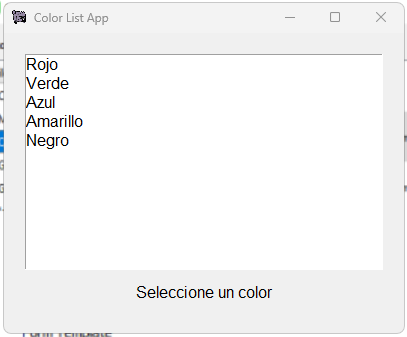
\includegraphics[width=0.6\textwidth]{img/Prueba01.png}
    \caption{Interfaz inicial de la aplicación Qt}
    \label{fig:qt_app}
\end{figure}

\begin{figure}[H]
    \centering
    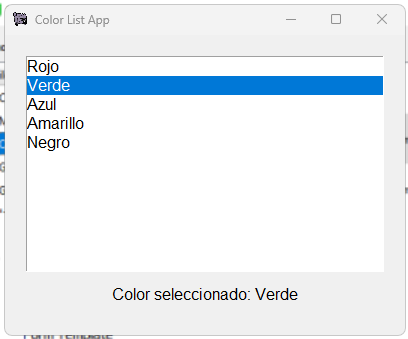
\includegraphics[width=0.6\textwidth]{img/Prueba02.png}
    \caption{Interfaz de la aplicación Qt después de seleccionar un color}
    \label{fig:qt_app_selected}
\end{figure}

\begin{figure}[H]
    \centering
    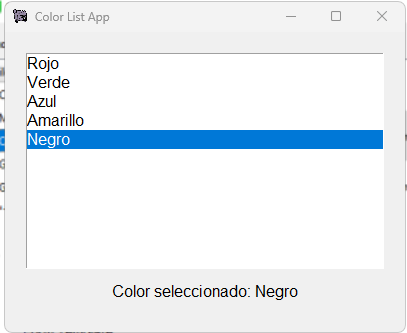
\includegraphics[width=0.6\textwidth]{img/Prueba03.png}
    \caption{Interfaz de la aplicación Qt después de seleccionar otro color}
    \label{fig:qt_app_selected2}
\end{figure}




\subsection{Actividad 02: Averiguar la implementación por signals y Slots, para comunicar los objetos del formulario del Task.ui (por ejemplo una caja de texto, o un Label) desde el MainWindows.h y CPP.}

En Qt, la forma correcta de comunicar widgets definidos en un archivo .ui con otra clase (por ejemplo MainWindow) es mediante el mecanismo de señales y ranuras (signals \& slots). Este sistema permite que los objetos se comuniquen sin depender directamente entre sí.

\begin{itemize}
    \item El Task.ui se convierte (por uic) en una clase Ui::Task con los punteros a los widgets (ej. lineEdit, label).
    \item Se crea una clase TaskForm que herede de QWidget y use esa UI.
    \item Se define un signal en TaskForm para avisar a MainWindow de cambios (por ejemplo, cuando el usuario escribe).
    \item Se define un slot para permitir que MainWindow actualice los widgets.
    \item En MainWindow, se conectan ambas partes con connect().
\end{itemize}

A continuación se muestra un ejemplo de cómo implementar esta comunicación entre TaskForm y MainWindow utilizando señales y ranuras en Qt.

\begin{lstlisting}[style=cpp-style, caption={TaskForm.h}]
#include <QWidget>
namespace Ui { class Task; }

class TaskForm : public QWidget {
    Q_OBJECT
public:
    explicit TaskForm(QWidget *parent = nullptr);
    ~TaskForm();

signals:
    void textChanged(const QString &text); // avisará al MainWindow

public slots:
    void setLabel(const QString &msg);     // llamado por MainWindow

private:
    Ui::Task *ui;
};
\end{lstlisting}

\begin{lstlisting}[style=cpp-style, caption={TaskForm.cpp}]
#include "TaskForm.h"
#include "ui_Task.h"

TaskForm::TaskForm(QWidget *parent) : QWidget(parent), ui(new Ui::Task) {
    ui->setupUi(this);

    // cuando el usuario escribe, emitimos la señal
    connect(ui->lineEdit, &QLineEdit::textChanged,
            this, &TaskForm::textChanged);
}

TaskForm::~TaskForm() { delete ui; }

void TaskForm::setLabel(const QString &msg) {
    ui->label->setText(msg);
}
\end{lstlisting}

\begin{lstlisting}[style=cpp-style, caption={MainWindow.cpp}]
#include "MainWindow.h"
#include "TaskForm.h"

MainWindow::MainWindow(QWidget *parent) : QMainWindow(parent) {
    auto *task = new TaskForm(this);
    setCentralWidget(task);

    // TaskForm -> MainWindow
    connect(task, &TaskForm::textChanged, this, [this, task](const QString &txt){
        task->setLabel("Texto: " + txt);
    });
}
\end{lstlisting}

\begin{enumerate}
    \item Usa signals para notificar eventos (de TaskForm a MainWindow).
    \item Usa slots para reaccionar o modificar el formulario (de MainWindow a TaskForm).
    \item Usa la sintaxis moderna de connect() (con punteros a miembros o lambdas).
\end{enumerate}


\subsection {Commits realizados}

\subsubsection {Primer Commit}

\begin{itemize}
    \item Este commit se hizo despues de terminar la primera implementación de código para C++ con Qt, 
\end{itemize}

\begin{figure}[H]
    \centering
    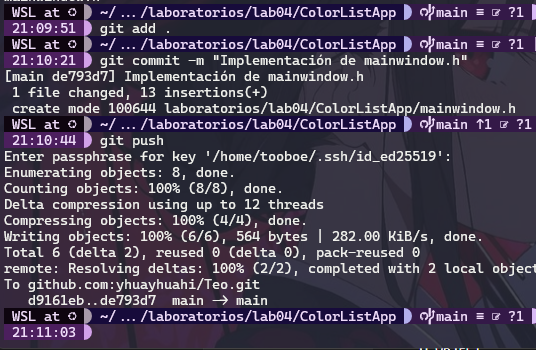
\includegraphics[width=0.8\textwidth]{img/Commit01.png}
    \caption{Primer Commit - Implementación en C++ con Qt}
    \label{fig:commit1}
\end{figure}


\subsubsection {Segundo Commit}

\begin{itemize}
    \item Este commit se hizo despues de terminar la implementación completa de código para C++ con Qt, despues de probar el funcionamiento.
\end{itemize}

\begin{figure} [H]
    \centering
    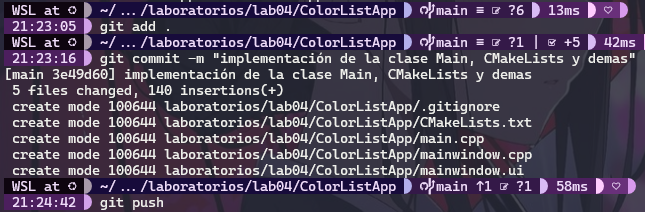
\includegraphics[width=0.8\textwidth]{img/Commit02.png}
    \caption{Segundo Commit - Implementación completa en C++ con Qt}
    \label{fig:commit2}
\end{figure}




\subsection {Estructura del laboratorio}

A continuación se muestra la estructura de archivos y carpetas del laboratorio realizado:
Claramente los archivos de compilación de Java y otros que se pudieron generar no se subieron al repositorio.

\begin{figure}
    \centering
    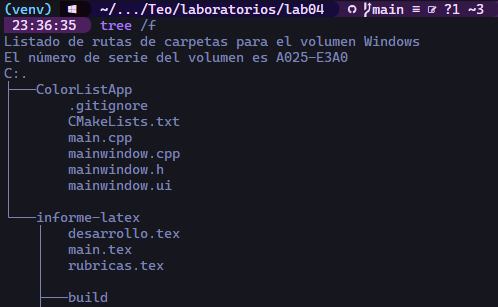
\includegraphics[width=0.8\textwidth]{img/EstructuraLaboratorio.png}
    \caption{Estructura de archivos y carpetas del laboratorio}
    \label{fig:estructura}
\end{figure}



\section{Cuestionario}

\textbf{No hay un cuestionario para este laboratorio.}




